\section{Grundbegriffe}
\subsection{Cloud}
Eine \textbf{Cloud} bezeichnet das Auslagern von Rechenaufgaben und Speicher auf
entfernte Computer, die nicht der eigene, lokale Rechner sind. Eine Cloud kann
unterschiedliche Aufgaben übernehmen; meistens sind es \textbf{Compute} (Rechenleistung)
und \textbf{Storage} (Speicher).
\subsection{Compute}
% LEKTORAT (Redundanz): Compute wird hier kanonisch erklärt. Die zuvor
% doppelte Compute-Erklärung in cloud_services.tex wurde entfernt.
\textbf{Compute} bedeutet im Cloud-Kontext, dass eine Cloud Rechenleistung
bereitstellt. Das kann auf vielfältige Weise geschehen: von einfachen
virtuellen Maschinen (VMs) über \textit{Managed Services} zum Hosten eigener
Anwendungen bis hin zu SaaS-Produkten wie \textit{Microsoft~365}.
\begin{figure}[H]
    \centering
    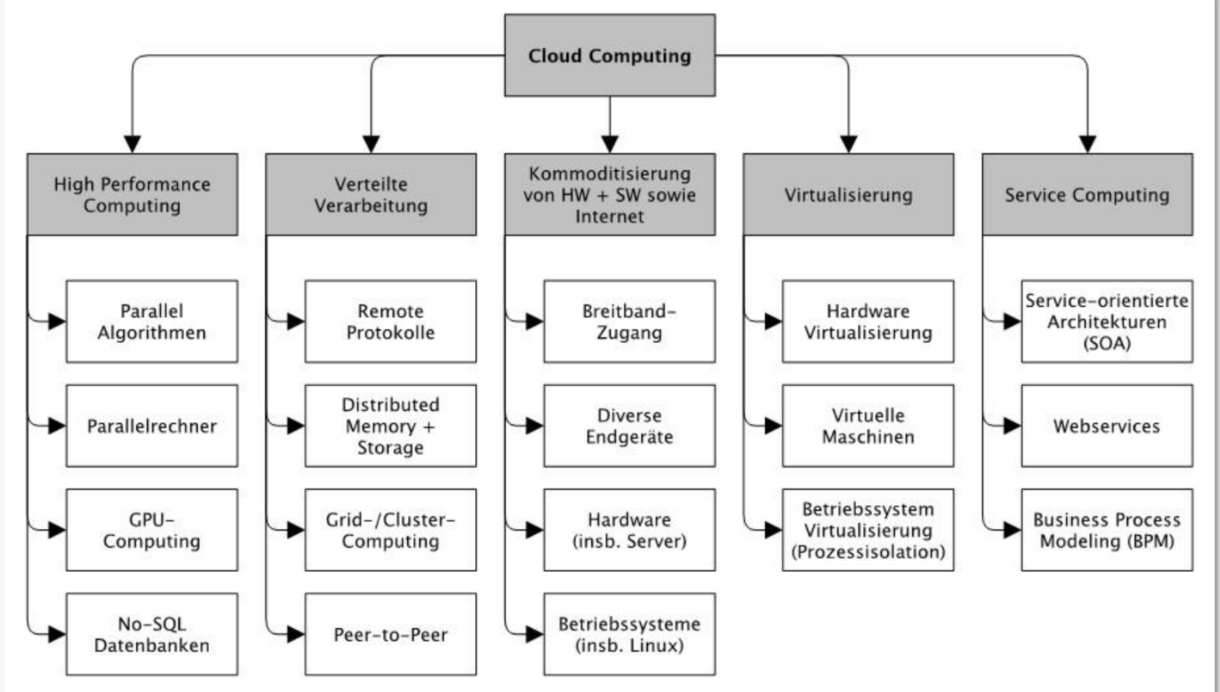
\includegraphics[width=\textwidth]{assets/images/CloudComputingErklaert}
    \caption{Cloud Computing erklärt}
\end{figure}
\subsection{Storage}
\textbf{Storage} bedeutet im Cloud-Kontext die Bereitstellung von Speicher. Auch das
kann auf unterschiedlichste Weise geschehen: als einfacher Cloud-Speicher
ähnlich einer Festplatte, als Speicher für Webanwendungen (etwa um Nutzerdaten
abzulegen) oder als Speicher, der in SaaS-Produkte wie \textit{Microsoft~365} oder
Streaming-Dienste wie \textit{Netflix} integriert ist.
